\documentclass[10pt,letterpaper]{article}
\usepackage[top=0.85in,left=2.75in,footskip=0.75in]{geometry}

% Use adjustwidth environment to exceed column width (see example table in text)
\usepackage{changepage}

% Use Unicode characters when possible
\usepackage[utf8]{inputenc}

% textcomp package and marvosym package for additional characters
\usepackage{textcomp,marvosym}

% fixltx2e package for \textsubscript
\usepackage{fixltx2e}

% amsmath and amssymb packages, useful for mathematical formulas and symbols
\usepackage{amsmath,amssymb}

% Use nameref to cite supporting information files (see Supporting Information section for more info)
\usepackage{nameref,hyperref}

% line numbers
\usepackage[right]{lineno}

% ligatures disabled
\usepackage{microtype}
\DisableLigatures[f]{encoding = *, family = * }

% rotating package for sideways tables
\usepackage{rotating}

% Remove comment for double spacing
\usepackage{setspace} 
\doublespacing

% Text layout
\raggedright
\setlength{\parindent}{0.5cm}
\textwidth 5.25in 
\textheight 8.75in

% Bold the 'Figure #' in the caption and separate it from the title/caption with a period
% Captions will be left justified
\usepackage[aboveskip=1pt,labelfont=bf,labelsep=period,justification=raggedright,singlelinecheck=off]{caption}

% Remove brackets from numbering in List of References
\makeatletter
\renewcommand{\@biblabel}[1]{\quad#1.}
\makeatother

% Leave date blank
\date{}

% Header and Footer with logo
\usepackage{lastpage,fancyhdr,graphicx}
\usepackage{epstopdf}
\pagestyle{myheadings}
\pagestyle{fancy}
\fancyhf{}
\lhead{
\includegraphics[width=2.0in]{PLOS-submission.eps}}
\rfoot{\thepage/\pageref{LastPage}}
\renewcommand{\footrule}{\hrule height 2pt \vspace{2mm}}
\fancyheadoffset[L]{2.25in}
\fancyfootoffset[L]{2.25in}
\lfoot{\sf PLOS}

%% Include all macros below

\newcommand{\lorem}{{\bf LOREM}}
\newcommand{\ipsum}{{\bf IPSUM}}

%% END MACROS SECTION


%%% Begin BWP
%\usepackage{amsmath, amsthm, amssymb, wasysym, graphicx}
%\usepackage[small, hang, bf]{caption}


%% CHOOSE!  Use PLOS idiot-biologist-content-free style, or
%% informative style for internal use?
% cite package, to clean up citations in the main text. Do not remove.
\usepackage{cite}
% Use the PLoS provided BiBTeX style
\bibliographystyle{plos2015}
\usepackage[normalem]{ulem}
%\usepackage{natbib}
%\bibstyle{plainnat}
%\renewcommand\cite{\citep}
%\newcommand\citepossessive[1]{\citeauthor{#1}'s \citeyearpar{#1}}

%\usepackage{polski} % For one dude's name in one bibliography entry!
%\usepackage[utf8]{inputenc}
%\a[lf]{berenis}
%\usepackage[LY1]{fontenc}

\newcommand\eq[1]{Eq.~\ref{#1}}
\newcommand\fig[1]{Fig.~\ref{#1}}
\newcommand\sref[1]{Section~\ref{#1}}
\let\oldmarginpar\marginpar
\renewcommand{\marginpar}[1]{\oldmarginpar{\linespread{1}\scriptsize{#1}}}

% PLOS wants \paragraph for some reason...
\renewcommand{\subsubsection}[1]{\paragraph{#1}}

\setlength{\marginparwidth}{55mm}


\newcommand\argmin{\mathop{\mbox{{\rm argmin}}}\limits}
\newcommand{\noprint}[1]{}

%%% End BWP


\begin{document}
\vspace*{0.35in}

% Title must be 250 characters or less.
% Please capitalize all terms in the title except conjunctions, prepositions, and articles.
\begin{flushleft}
{\Large
  \textbf\newline{A Multi-Channel Electrode for Chronic Recording and Safe Current-Steered Stimulation}
}
\newline
% Insert author names, affiliations and corresponding author email (do not include titles, positions, or degrees).
\\
Ben Pearre\textsuperscript{1,a,\textcurrency},
Sanne~Moorman\textsuperscript{1,b},
Jun Shen\textsuperscript{1,c},
Stuart F.~Cogan\textsuperscript{2,d}
Timothy J.~Gardner\textsuperscript{1,e}
\\
\bigskip
\textsuperscript{1} Department of Biology, Boston University, Boston, Massachusetts, United States of America\\
\textsuperscript{2} Department of Bioengineering, University of Texas, Dallas, Texas, United States of America
\\
\bigskip

% Insert additional author notes using the symbols described below. Insert symbol callouts after author names as necessary.
% 
% Remove or comment out the author notes below if they aren't used.
%
% Primary Equal Contribution Note
%\Yinyang These authors contributed equally to this work.
Author \textsuperscript{a}~did something, we think.  The histology data analysis was by Author \textsuperscript{b}. Author \textsuperscript{c} performed all surgeries.  Authors \textsuperscript{b} and \textsuperscript{c} did the histologies.  Author \textsuperscript{d}, the PI, designed and guided the experiment and this paper.

% Additional Equal Contribution Note
% Also use this double-dagger symbol for special authorship notes, such as senior authorship.
%\ddag These authors also contributed equally to this work.

% Current address notes
%\textcurrency a Insert current address of first author with an address update
% \textcurrency b Insert current address of second author with an address update
% \textcurrency c Insert current address of third author with an address update

% Deceased author note
%\dag Deceased

% Group/Consortium Author Note
%\textpilcrow Membership list can be found in the Acknowledgments section.

% Use the asterisk to denote corresponding authorship and provide email address in note below.
\textsuperscript{\textcurrency} Corresponding author: bwpearre@gmail.com (BP)

\end{flushleft}

\reversemarginpar
%%% End PLOS header template



\begin{abstract}

Electrical control of the brain facilitates a variety of therapeutic and scientific goals, from treating sensory, motor, and cognitive defects to exploring the effects of disrupting or subtly modifying the brain's behaviour in real time.  These procedures are limited by the brain's reaction to foreign matter: over a period of months, glia encapsulate the electrodes, isolating them from neurons, allowing monitoring and control of the brain only over large spatial scales---often on the order of millimeters.  Small electrodes ($<$ 10 $\mu$m) minimise encapsulation, and thus can both record single neurons for many months and precisely stimulate small groups of neurons.  However, the high impedance of small electrodes can require stimulation voltages that exceed the water hydrolysis point.

We have developed an electrode design in which groups of electrodes support each other during insertion and then splay randomly in the brain, allowing long-term small-spatial-scale recording and stimulation.
  
  We describe the splaying properties of these electrode arrays in the brain.  We present preliminary results showing that these electrodes remain capable of recording individual spikes for a year after implantation, even when also used to stimulate.

  We present preliminary evidence that the spatial scale of the splaying is sufficient to allow the steering of current between the electrodes, and that this allows a degree of high-dimensional control over the brain's response to stimulation.  We show that appropriate control of the electrode array can produce neural responses while keeping stimulation voltages below safety limits.  Furthermore, we demonstrate controllable differentiation between responses, even in an upstream brain area.

  Thus these multichannel, spatially distributed, micron-scale arrays allow long-term single-unit recordings, enabling new experiments investigating how the brain changes on long timescales.  In addition, current-steered control of stimulation inputs allows fine-grained control over small groups of neurons, permitting a wide variety of optimisations, such as controlling the brain to some set of desired responses, or minimising the voltage or energy required in order to achieve the desired result.

\end{abstract}

\linenumbers

\section{Introduction}

Goal: controlling the brain.

How it's done now: large electrodes, coarse stimuli, crude if any feedback control (due to large electrodes), poor control due to imprecision of stimulation.

How we want to do it: small electrodes that splay.
\begin{itemize}
\item Small size permits chronic single-unit recording, but delicate.
\item Bundled, they are strong enough to implant.
\item Current steering may overcome stimulation current and voltage restrictions.
\item Small size, splayed geometry, high channel count allow a new frontier in fine-grained control.
\end{itemize}


\subsection{Review of electrode size and damage}

{\em Large electrodes must be stimulated at high currents.  Energy inefficiency.  Imprecision.  Sense-act cycles are limited.}

Electrodes with cross-sectional dimension above about 10 $\mu$m result in glial scarring up to 300 $\mu$m from the implant (and \cite{Butson2008steering} assumes a 500-$\mu$m encapsulation layer for the $\sim$ 1.3-mm electrodes common in DBS), tissue damage, ever-increasing stimulation thresholds, unable to record from some cell types \cite{Biran2005gliosis,Polikov2005gliosis,Winslow2010gliosis}. 

Recording is limited by gliosis / encapsulation.  This is mitigated by electrodes $<$ 10 $\mu$m, but these present two difficulties: they are too weak to insert, and during stimulation, their small surface area requires high voltage in order to deliver sufficient current to induce response.

Our hexadecode \cite{Guitchounts2013electrode} uses multiple shanks each of which is too small to stimulate adverse tissue reactions.  The shanks are bundled to support each other during insertion.  They splay in the brain, giving randomly distributed sites for recording and stimulation.


\subsubsection{Charge injection}

In order to increase the charge injection capacity of our electrodes, we tried electroplating them with iridium oxide.  This effected an improvement of roughly an order of magnitude: impedances went from around 2 M$\Omega$ to 200 k$\Omega$, and for a given current, the required voltage was much lower.\marginpar{FIXME}  We also experimented with PEDOT, which has excellent charge-injection properties, but we found it to have durability issues.\marginpar{All I know about this is hearsay.}  See \cite{Cogan2008electrodes} for a review of electrode physics.

\subsection{Review of current steering}

\subsubsection{Deep Brain Stimulation}

Much of the work in current steering in the brain is due to the interest in deep brain stimulation (DBS).  Electrodes tend to be single rods 1.2--1.6 mm in diameter with 4--32 contacts.

DBS has been used to treat movement disorders (especially those associated with Parkinson's disease), epilepsy, Alzheimer's, chronic pain, cluster headache, depression, OCD, addictive behaviours, anorexia\dots\marginpar{Many more!  But do we want to provide a big list?  Only if we are selling this as a clinical paper, right?}

Most\marginpar{Review what's known of DBS's mechanisms of action?  Perhaps only marginally relevant, but there's a good review in \cite{Udupa2015dbs}.} attempts to steer current use computational models of brain tissue to predict current-steering configurations that preferentially target the intended type of tissue, or make up for errors in electrode placement during surgery \cite{Holloway2005stereotaxy}.  One approach \cite{Butson2008steering,Chaturvedi2012} builds a model of the tissue of interest using magnetic resonance imaging (MRI) and diffusion tensor imaging (DTI) \cite{Tuch2001conductivity,Alexander2007dti}, which produces data with voxels of roughly 2 mm\textsuperscript{3}.  They then use 3D finite element analysis to predict current steering trajectory.\marginpar{Lots more references might be added here, all of which have spatial resolution on this order and a variety of temporal resolutions; choose $\approx$3 or just cite a review?}

Current-steered and adaptive DBS have been shown 

\subsubsection{Current steering on a smaller scale:}

\cite{Jepson2014steering_in_retina} use 64-channel electrode arrays, with electrode as closely packed as 30 $\mu$m, to stimulate macaque retina {\em in vitro}.\marginpar{Note about how different retina structure is from our areas?}  They stimulated the retina using single electrodes or combinations of three electrodes with charge-balanced pulses, and found that retinal response could be predicted with a piecewise linear model.


\subsubsection{Something?}

Efforts to steer current outside of the brain have also been pursued,\marginpar{Sounds so weak!  Turn this into a bigger review?} \cite{king2006current_steeriing_optimisation} describes an algorithm for clinician-assisted search for effective stimulation in multielectrode arrays in the spinal cord.  The patent defines an algorithm for hillclimbing search, controlled by a clinician.  \cite{parramon2011current_steering_optimisation} develops an even more creative specialised hillclimbing search method.  However, we have not seen application of standard optimisation techniques in this domain.

\subsection{Stimulation: closing the loop}

Standard DBS systems deliver some kind of stimulation continuously.  Recently, interest in using biological feedback has grown.  Due to the size of the electrodes, for feedback control most systems rely on large-spatial-scale metrics such as local field potentials (LFP) \cite{Priori2013adbs-lfp} and other macroscopic measures of outcome such as surface electromyography\marginpar{Basu, ``Pathological tremor prediction using surface electromyogram and acceleration''} and accelerations \cite{Afshar2012closedloop}\marginpar{Great review: \cite{Priori2015review}} but the addition of a second electrode in a different brain region has been shown to be effective in ameliorating Parkinsonian symptoms in monkeys \cite{Rosin2011adbs}.


\subsection{Contribution}



\section{Materials and Methods}

\subsection{Bird surgery description}

Jun?

Ground/return electrode should be described somewhere.  Here?


\subsection{Electrode construction}

Electrode arrays were constructed as described in
\cite{Guitchounts2013electrode}.  The charge transfer capacity of one
of the stimulation electrodes was enhanced by electrodeposited iridium
oxide.  \cite{Cogan2008electrodes} describes the electrochemistry of
charge transfer.

\subsection{Splay histology}

Electrode bundles were implanted into birds, all to a depth of roughly 3 mm.  Most of these were ``dummy'' uncoated and blunt-cut rather than fire-sharpened as in \cite{Guitchounts2013electrode}, with 10--16 channels (fibres).  The birds were killed, and their brains sectioned roughly perpendicularly to the electrodes, with a slice thickness of 50 $\mu$m.\marginpar{Sanne: what slice thickness?}

The following criteria were used to exclude observations:\marginpar{Sanne: check exclusion criteria.}
\begin{itemize}
\item Individual fibres were excluded if they were lying flat on the surface of the tissue (visible as side-on cylinders).
\item Bundles were excluded if they were implanted in fibres of passage.
\end{itemize}


Clustering was done by hand.  The set of distances between electrodes was computed by measuring the distance between each electrode and its nearest neighbour.\marginpar{I'm about a day from finishing software to do all-to-all comparison.  For the draft (and possibly first submission, if time is tight) this suffices.}  Bundles were clustered as follows:
\begin{description}
\item[Splayed:] All electrodes were more than 10 $\mu$m from each other, or at most one pair was closer.\marginpar{Why 10 $\mu$m?}
\item[Partial:] Some \marginpar{How many?} electrodes were more than 10 $\mu$m from each other.
\item[Clumped:] All electrodes were within 10 $\mu$m of each other.  \marginpar{All-to-all, or nearest-neighbour?}
\end{description}
\par\noindent Examples of these three categories are shown in \fig{fig:splay_montage}.

\begin{figure}
  % montage -geometry 1024x1024 splay_full.jpeg splay_partial.jpeg splay_no.jpeg splay_montage.eps
  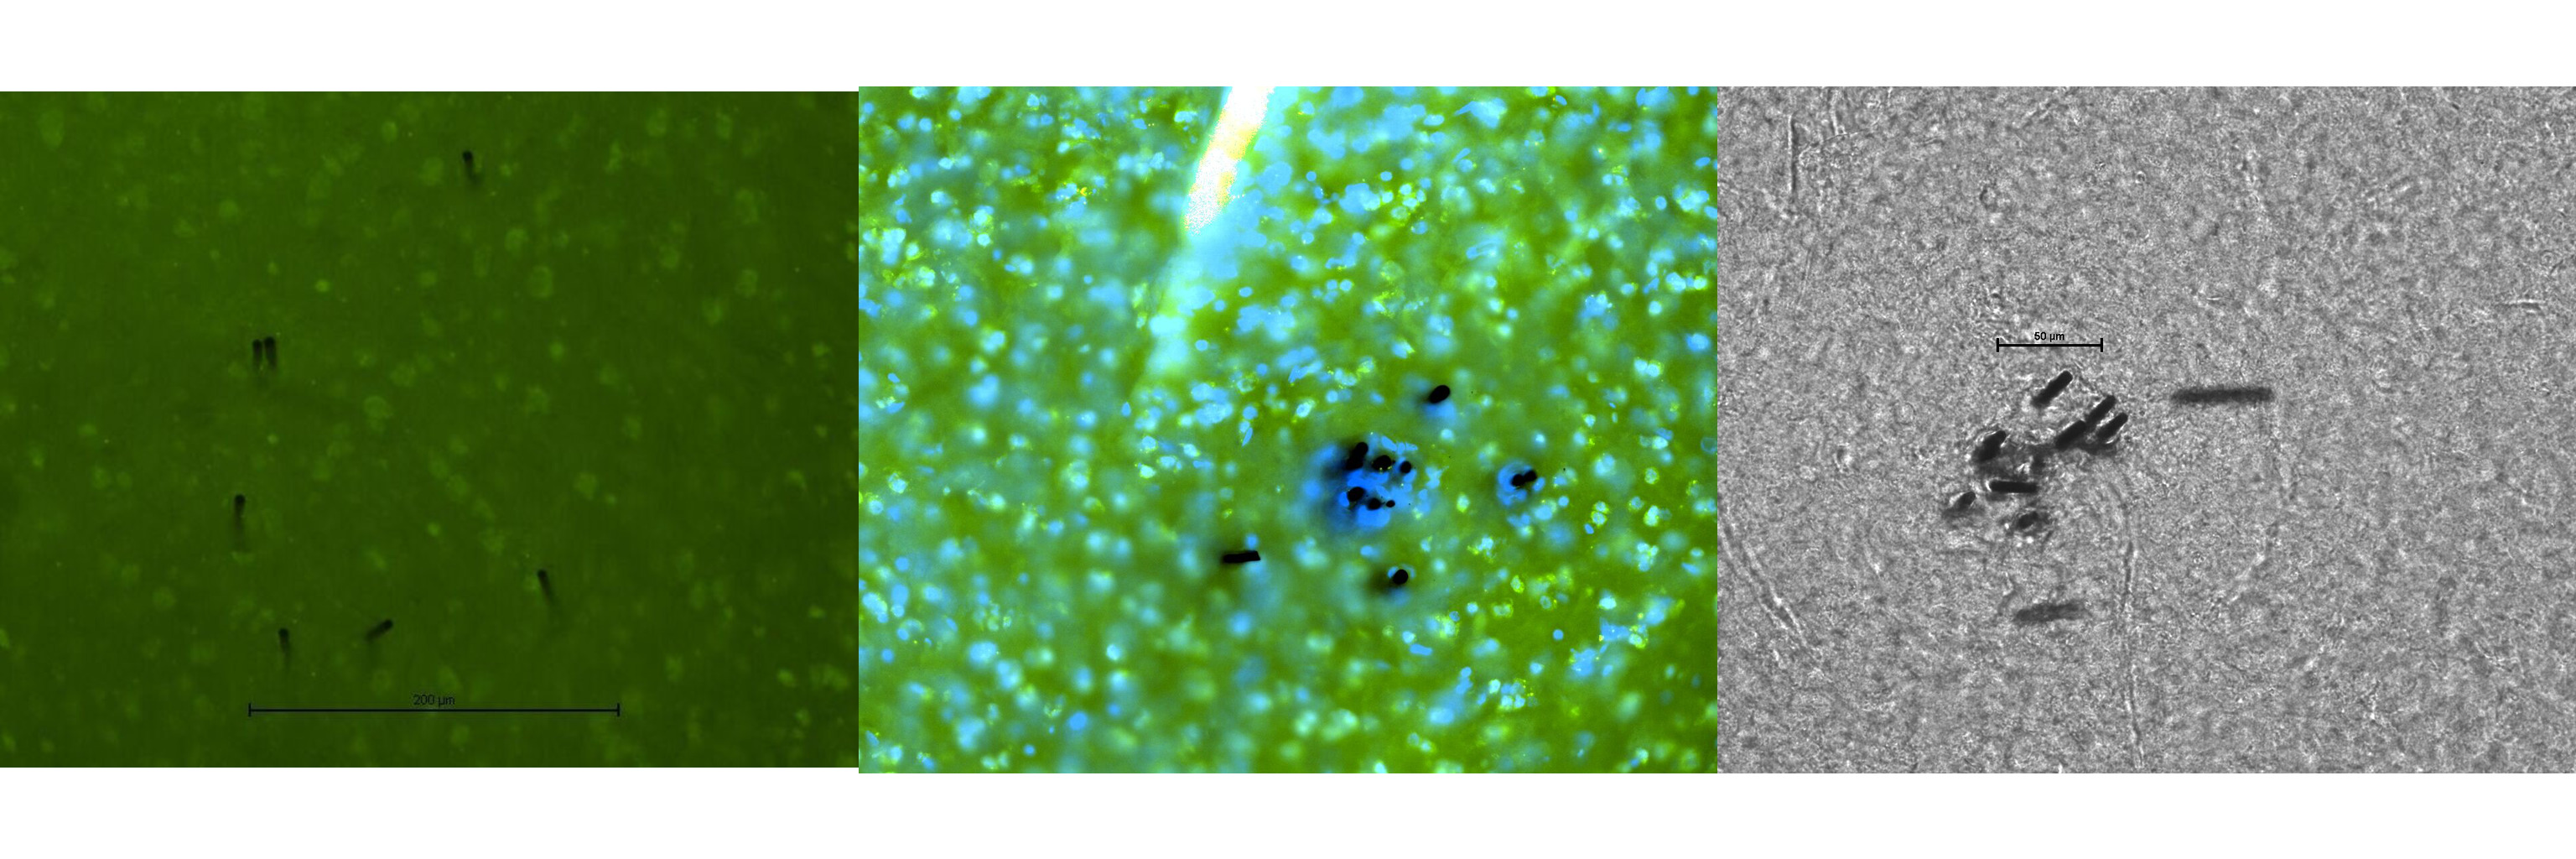
\includegraphics[width=\textwidth]{splay_montage}
  \caption{Splay types, left to right: examples of full splay, partial splay, and clumped.  In all images, black circles are electrode shafts; in many cases the slicing plane is not quite orthogonal to the electrodes, yielding oblong images.  In the bright-field image on the right, three of the electrode slices were pulled out of the tissue during slicing, and appear to lie flat on the slide.  Since their original locations cannot be determined, we have ignored them.}
  \label{fig:splay_montage}
\end{figure}

\marginpar{Would it make sense to automatically cluster the splay data?  Or to change the criteria?  I can think of some changes\dots}


\subsection{Recording}

Recordings of spontaneous activity were done using an Intan RHD2000 amplifier at 20 kHz, with a hardware high-pass filter at 200 Hz.

\subsection{Stimulation: Zebra finch antidromic HVC $\leftarrow$ X}

A common technique for locating HVC in the zebra finch involves implanting a stimulating electrode in Area X and looking for a an antidromic response \cite{Swadlow1998antidromic,Hahnloser2002sparse}, which is visible in HVC but not in the surrounding tissue.

Electrical stimulation saturates the brain, including the recording
electrode, for some time post-stimulation (depending on the hardware
used, but generally 1--3 ms post-stimulation).  Responses to
stimulation can be detected outside of that saturation window.

We tested our ability to steer current in the brain by stimulating in
Area X and monitoring the response in HVC, about 5 mm away.  This
spatial separation results in synaptic transmission delays of between
3 and 8 ms \marginpar{Tim: citation for 3--8 ms?}, which gives the
recording amplifier time to settle before measuring the
response.\marginpar{But why antidromic?}

We will use the following definitions:

\begin{description}
\item[Channel:] Our electrodes have 16 separate carbon fibres, each one of which we consider a separate channel, since each is connected to a separate amplifier.  Some work better than others, and usually about 75\% of them have low enough impedance to use.  We refer to these as active channels, or just channels.
\item[Pulse:] A biphasic charge-balanced square wave of current.  Each phase is 200 $\mu s$ long, and there is no interpulse interval.
\item[Current-steering configuration (CSC):] The configuration defining which channels receive the positive half of their biphasic pulse first, or vice versa.
\item[Pulse train:] A sequence of 10 identical pulses delivered simultaneously to all active chennels at 25 Hz.  This is slow enough that pulses do not interfere with each other, and is used to detect the reliability of the response.
  \begin{itemize}
  \item Programming\marginpar{Move timing notes to Discussion of compromises required for this experiment?} the Plexon stimulator for one pulse train requires about 2 seconds.
  \end{itemize}
\item[Threshold scan:] A series of pulse trains, each of which has the same CSC but a different current, designed to find the minimum current for this CSC that will antidromically induce a response in HVC.  The algorithm is described below.
  \begin{itemize}
  \item A threshold scan generally requires roughly 15 pulse trains, and thus takes on the order of 30 seconds.
  \end{itemize}
\item[Voltage scan:] The Plexon hardware can deliver a current-controlled pulse to each of 16 channels independently, but only allows monitoring of the voltage delivered on one channel at a time.  A voltage scan involves sending the same pulse train once per active electrode, monitoring a different one each time.
  \begin{itemize}
  \item A \marginpar{This does not require full reprogramming of the Plexon!  Just setting the monitor channel is faster, but my code does not take advantage of this, and fully reprogrammes the Plexon each time.} voltage scan requires delivering one pulse train per active electrode, taking a total of about 30 seconds.
  \end{itemize}
\end{description}

The stimulation and recording electrodes use separate electrical returns, consisting of\marginpar{Jun?} silver wire in contact with the skull.  Some CSCs balance current delivery between the electrodes, whereas others do not, and in the latter case excess current flows through the common return.

We used a Plexon stimulator to control stimulation in Area X, and recorded from HVC using a Tucker-Davis Technologies RZ5 amplifier\marginpar{And/or an Intan, depending on which recording to show in \fig{fig:clear_hvc_response}}.  The Plexon self-monitoring channels were recorded on a National Instruments PCI-6251 data acquisition card using the session-based interface of Matlab (various versions from 2014a through 2015b) on Windows 8.1.

We used MATLAB to control the stimulation and acquisition as follows: the National Instruments card is set to record an adequate number of samples of the Plexon self-monitoring channels at 100 kHz, initiated through software, and sending out a TTL pulse at the beginning of acquisition.  The Plexon stimulator begins stimulating upon receipt of that TTL pulse, and the TDT begins recording at 24.414 kHz (the device's native frequency) on the same signal.  Whenever the Plexon is actively delivering current (i.e. during each pulse within the train) it sends out its own TTL pulse: this signal is recorded by the TDT along with the HVC electrode voltages in order to align stimulation pulses with the recording.  The alignment precision is limited only by the sampling rate of the TDT.

\subsubsection{Response detection}

HVC projects into Area X (and into RA, which we do not discuss here).  When Area X is stimulated, an antidromic response may be observed both in HVC\textsubscript{X} projection neurons and in HVC interneurons.  The antidromic response occurs roughly 3--8 ms after the stimulation pulse,\marginpar{Citation!} and is highly stereotyped: \cite{Fee2004mechanisms} reports that the variability in the timing of the antidromic response in HVC\textsubscript{X} projection neurons is under 50 $\mu$s, while that of HVC intraneurons is above 500 $\mu$s.

\fig{fig:clear_hvc_response} shows an example of a pronounced HVC response to stimulation in Area X.  In order to detect this signal, we measure the cross-correlation between the recorded response for each pulse in a train and each other with a maximum lag of 50 $\mu$s, which provides a robust way of separating neural response from noise.  Because the HVC amplifier's response to the transient stimulation pulse in Area X can persist into the time of interest (3--8 ms), each response is first de-trended using a maximum-likelihood fit over the region 2--25 ms using an eigth order Fourier Series, which removes post-stimulation decay while leaving intact spike-sized signals.\marginpar{Filtering would probably work better with the TDT\dots}  We found this to produce fewer artifacts than the more conventional approach of bandpass-filtering the signal, given the large stimulation artifact.  The cross-correlation threshold above which a response is identified is chosen by visual inspection.\marginpar{But now why not findpeaks $3\sigma$ or whatever, and see if peak jitter is $<50\mu$s as required by \cite{Fee2004mechanisms}?  This has the great advantage that over an $n$-spike train, I could immediately compute Pr(response) (see marginpar QWE to see why this is a good idea).  Could reanalyse old data this way and compare, and decide whether to go forward.}

\begin{figure}
  \includegraphics[width=\textwidth]{lw95rhp-2015-08-05_18.39.07.eps}
  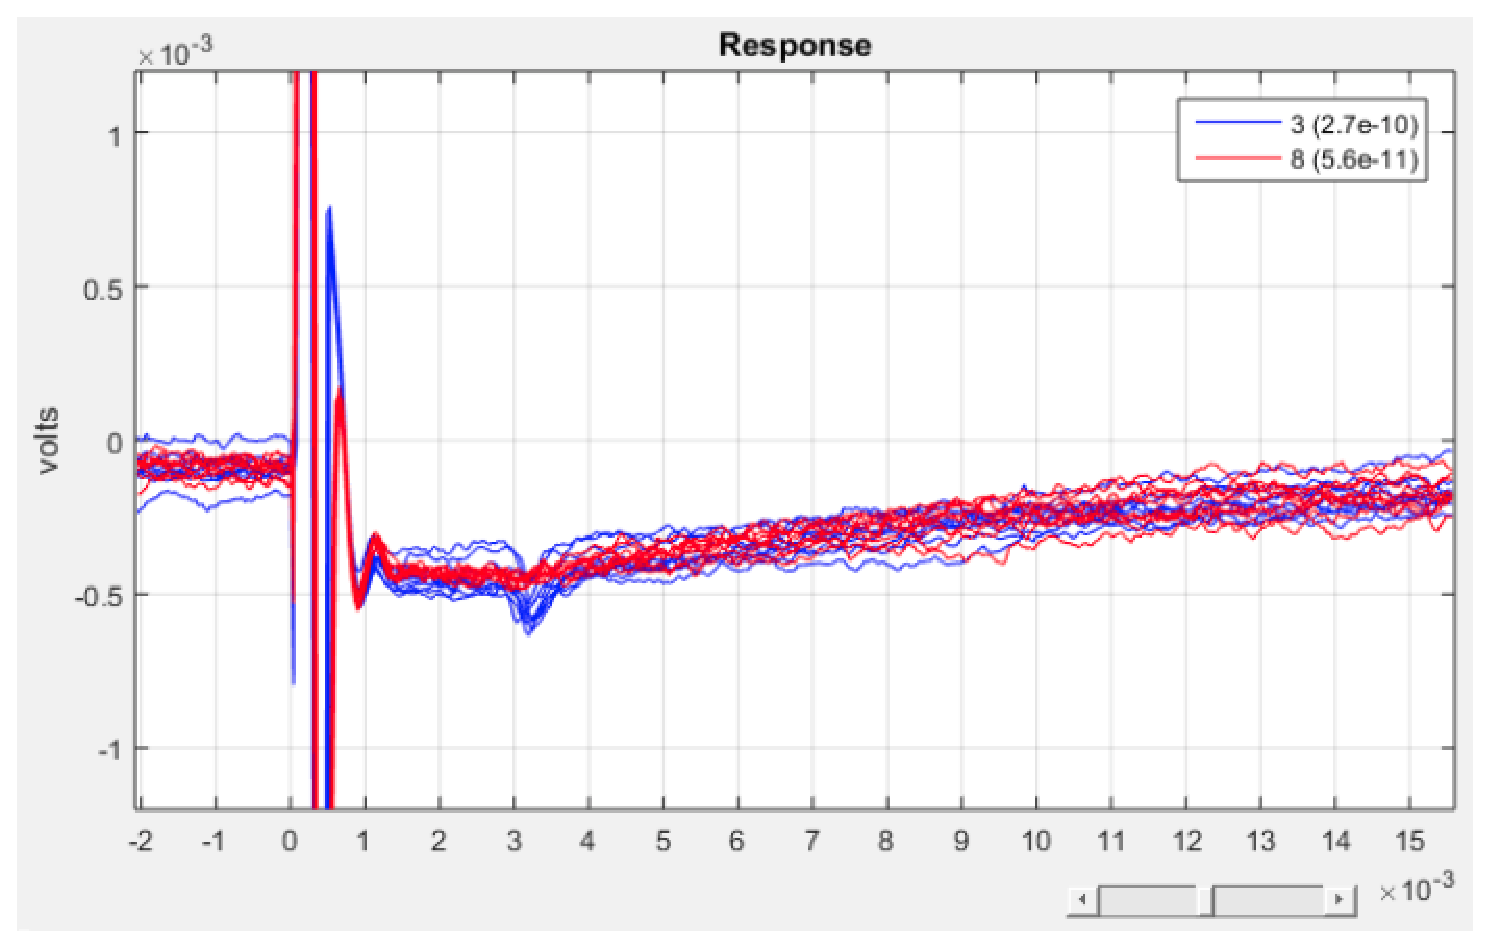
\includegraphics[width=\textwidth]{lw95rhp-2015-12-02}
  \caption{An example of a strong response in HVC.  {\bf Top:} The horizontal axis is time in milliseconds relative to the onset of a stimulation pulse.  Here, the stimulation is a 400-$\mu$s biphasic pulse of 3 $\mu$A, in which voltage peaked at 1.6 V.  Stimulation was repeated 20 times at 25 Hz, with each response aligned to its respective pulse.  Various response activity can be seen, but the most pronounced is at 6.2 ms post-onset.  {\bf Bottom:} a different bird, with a much weaker signal, but recorded on TDT.  200 $\mu$s, 6.94 $\mu$A, 1.2 V peak.{\em Use the top figure?  It only shows one channel, and it's recorded on the Intan, which I was using while the HVC signals were still pretty.  That means a lot worse amplifier settling, so it's not the best image, but the response is much cleaner than later ones made with the TDT.}}
  \label{fig:clear_hvc_response}
\end{figure}

As the bird ages, the skull grows down from the implantation site.  For shallow installations such as HVC (depth $\approx 200\mu m$, the quality of the HVC recordings diminishes as electrodes are forced out of contact with the brain.  This makes it more and more difficult over time to measure the antidromic response.  The above cross-correlation technique is more sensitive than the technique typical of acute or short-term response measurements, in which a pronounced spike is often clearly visible.\marginpar{Need to prevent antidromic response transmission and see if ``measured response'' disappears as it should!  But this requires more birds, and a more complex experiment.} We believe that we are measuring an antidromic response because it is on the correct timescale and appears near the expected stimulation threshold.\marginpar{Cite papers giving timing and stimulation threshold.}

\subsubsection{Threshold scan}

What stimulation parameters are required in order to reliably elicit an antidromic response to stimulation in Area X?  How can this threshold be found quickly, while minimising the risk of exceeding safe stimulation voltages?  How can this process be made robust to noise?\marginpar{How can we establish how much robustness to noise is required?}

After choosing a CSC,\marginpar{Perhaps write a pseudocode block instead of this mess?} we begin stimulating at a current that is known to be below threshold.  While no response is seen, the current is increased gradually (by a factor of $\alpha \approx 1.1$) until either a response is detected or the voltage or current limit is exceeded.  In the latter case, a lack of response is reported, and we move on to the next CSC.  If a response is found, then the step size is decreased ($\alpha \leftarrow \alpha^{2/3}$) and we reduce the current until the response disappears.  This process is repeated until the step size drops below a limt ($\alpha < 1.02$), and the threshold is taken as the last parameter set that induced a response.

A further, independent analysys was performed on the data set: for each pulse train, spikes were detected by looking for peaks greater than 5 standard deviations from the RMS noise of a nearby non-stimulated sample on the same electrode.  The peaks' delays post-stimulus were compared, and any peak whose delay was within 100 $\mu$s of another peak was considered a response to the stimulus.  The probability of a response at this current was then the maximum number of aligned peaks divided by the number of pulses in the train.  Given the set of points Pr(response$\,\,|\,\,$maximum electrode voltage), we then fit a sigmoid $0.5 + 0.5 \tanh(\lambda(x-\mu))$ to this curve, and take the midpoint $\mu$ as an alternative measure of the voltage required to induce a response with probability 50\%.\marginpar{Search could even be conducted as above (although could do better) or terminated by estimating the error on the estimate.}

While a larger step size would result in a faster search, and a binary search would be easier to describe, this ad-hoc approach samples near the current of interest while making it unlikely that we will stimulate with a current that significantly exceeds the minimum required for a response, and thus minimises the possibility of injuring the bird.

\subsubsection{Voltage scan}

Once the minimum current required in order to achieve a response is identified, we perform a voltage scan at that current, in order to measure the peak voltage delivered to each electrode.

\section{Results}

\subsection{Splay histology}

After exclusion, 22 arrays, implanted into 13 different birds, each yielded at least 3 measurable electrodes.  See Table~\ref{table:splaydata} for the raw data and \fig{fig:splaydata} for visualisations thereof.\marginpar{Perhaps take out the table and just use the graphs?}



\begin{table}
  \begin{tabular}{cccc}
    & \multicolumn{3}{c}{Inter-electrode distance ($\mu$m)} \\
    \# Good electrodes & Mean & StdDev & Max \\
    \hline
     3  &  5.0    &    0 &  20.0 \\
   10  &  6.0   & 2.1 &  52.9 \\
   16  &  6.3   & 6.3 &  48.3 \\
    4  &  7.5   & 5.0 &  35.8 \\
    6  & 16.7  & 18.9 &  44.8 \\
    9  &  7.7   & 5.5 & 107 \\
   14 &  12.8  & 12.1 & 15.2 \\
    8 &  14.7  & 17.8 & 108 \\
   15&   15.1  & 10.2 & 163 \\
   15  & 19.3  & 19.1 & 128 \\
    5  & 22.0  & 27.7 & 103 \\
    9  & 28.2   & 35.8 & 148 \\
   11 &  31.8  & 28.1 & 103 \\
    8  & 35.9  & 30.6 & 228 \\
   13 &  76.5 & 152 & 167 \\
    5  & 51.4  & 28.1 &  51.5 \\
    3  & 20.0    &     0 & 123 \\
    6  & 73.5  & 35.5 & 128 \\
    8  & 38.5  & 35.2 & 142 \\
    9  & 47.4  & 31.5 & 208 \\
    5 & 126  & 63.5&  214 \\
    16 &  62.0 &  58.9&  829
  \end{tabular}
  \caption{Raw data.  Each row shows the statistics from one electrode array.  ``Good'' electrodes is the the number of carbon fibre electrodes in each bundle that appeared to still be firmly fixed in the neural tissue after slicing.}
  \label{table:splaydata}
\end{table}

\begin{figure}
  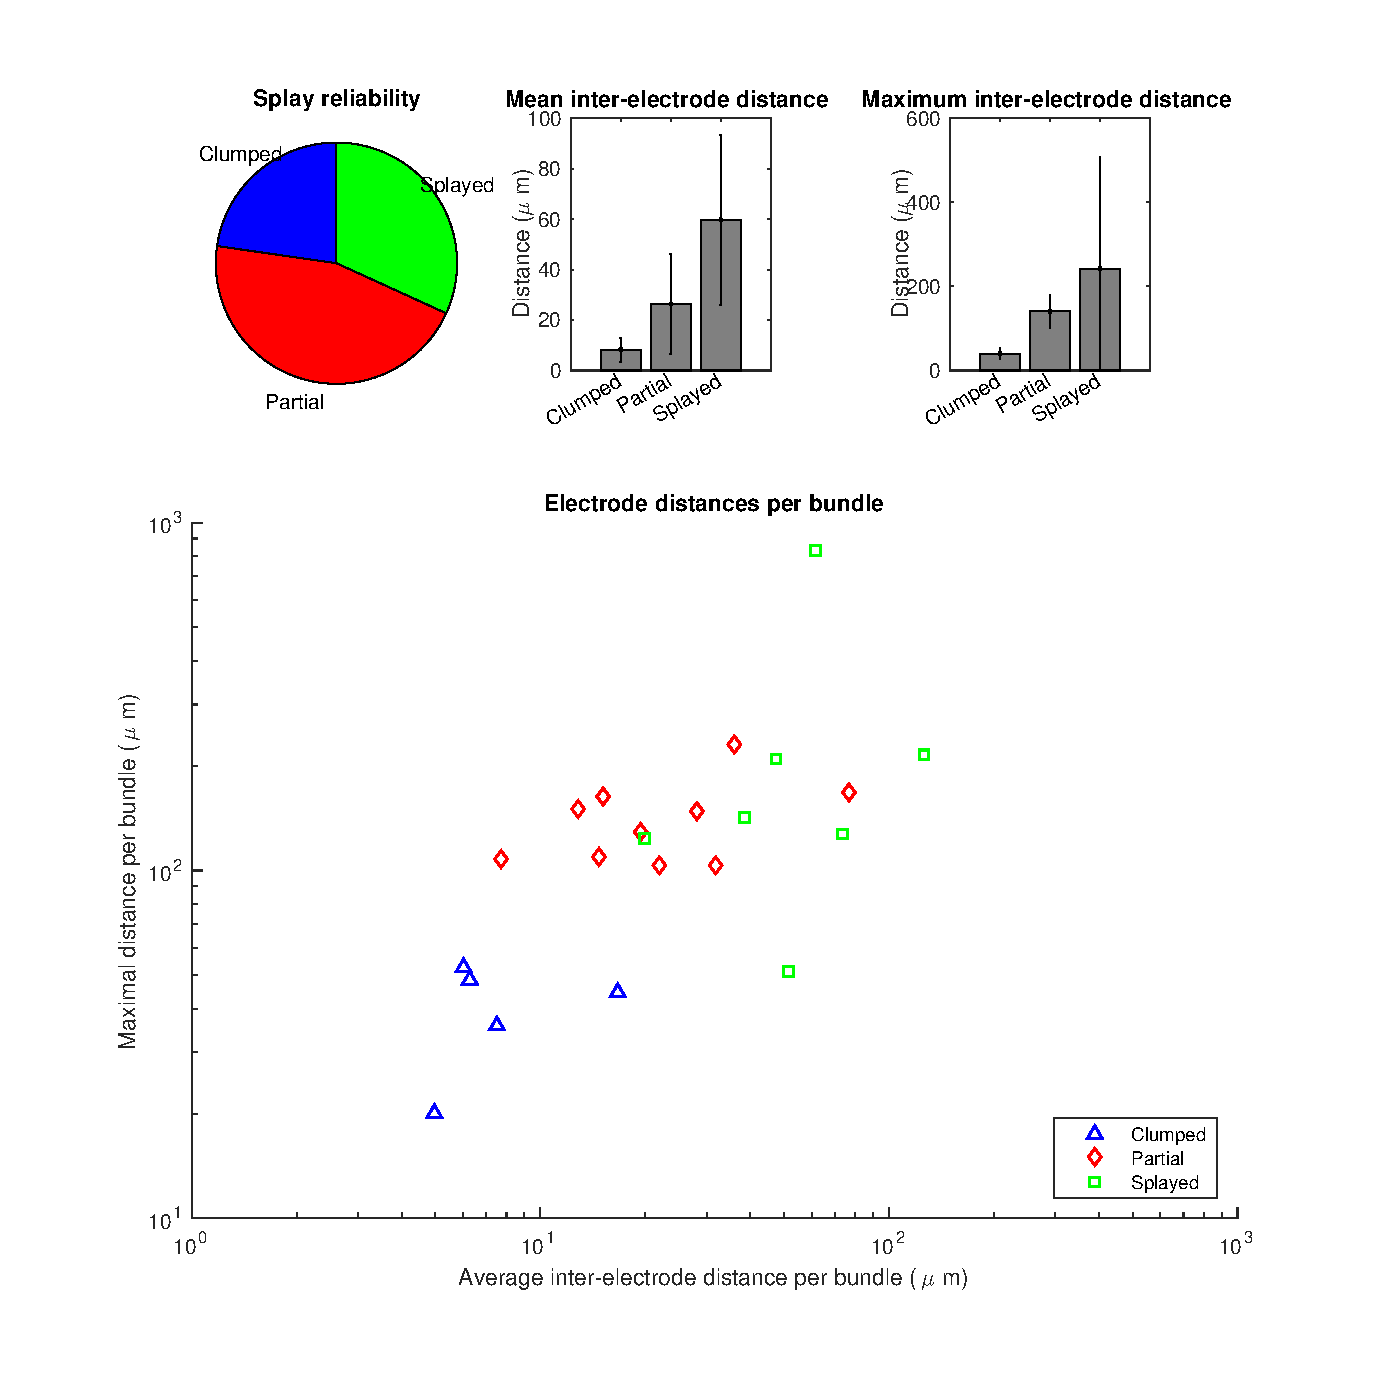
\includegraphics[width=\textwidth]{splay_data}
  \caption{Splay histology data from Table~\ref{table:splaydata}.}
  \label{fig:splaydata}
\end{figure}

\fig{fig:damage} shows some examples of the damage done to the brain in the vicinity of tle electrodes.\marginpar{An image of ``typical'' damage done by ``micro''electrodes would be nice, but it's hard to show what's typical of the \sout{competition} prior work with any credibility.  Letting people compare vs.~their own experiences is the best, but not everyone (e.g. me) will know what's typical.}
\marginpar{I have data on how long post-implant the birds lived, which needs to come along with this figure, if not the rest of the paper.} Visual inspection shows little damage in the vicinity of single electrodes, and slightly more in clumped electrode groups.  Visual inspection can give some indication of the damage done to the brain and the likelihood of achieving good electrical contact with neurons, but we are more interested in the ability to record signals (see Section~\ref{sec:results:recording}).

\begin{figure}
  % montage -geometry 1024x1024 DAPI-and-NeuN*.jpeg damage.eps
  \includegraphics[width=\textwidth]{damage}
  \caption{Damage.  Neural nuclei are shown in green (stained with NeuN) and all cells in blue (DAPI).  The presence of non-neural cells indicates damage, and is notable in the vicinity of the largest non-splayed electrode bundle, and nearly absent around individual electrodes.}
  \label{fig:damage}
\end{figure}




\subsection{Chronic recording}
\label{sec:results:recording}

\subsubsection{Impedances}

\marginpar{Need a graph showing impedances per electrode over time.  At least I have data for that; just haven't writtent the code to extract+plot.}

\subsubsection{HVC}

Long-term recording in HVC is difficult due to skull regrowth interfering with electrodes implanted only a few hundred microns from the surface: after 10 months, we had difficulty picking up antidromic response in our two remaining birds.

\subsubsection{Area X}

More telling of the potential of these electrodes is the recording of spontaneous activity in Area X, which was still easily seen in several channels after a year.\marginpar{I don't have recording-only data from early on.}   \fig{fig:XSpikeRecording} shows recordings in the weeks leading up to the 1-year mark.  These are the three most stable electrodes of the 16.



\begin{figure}
  % Width 9, Height 9, Font scaling 100%
  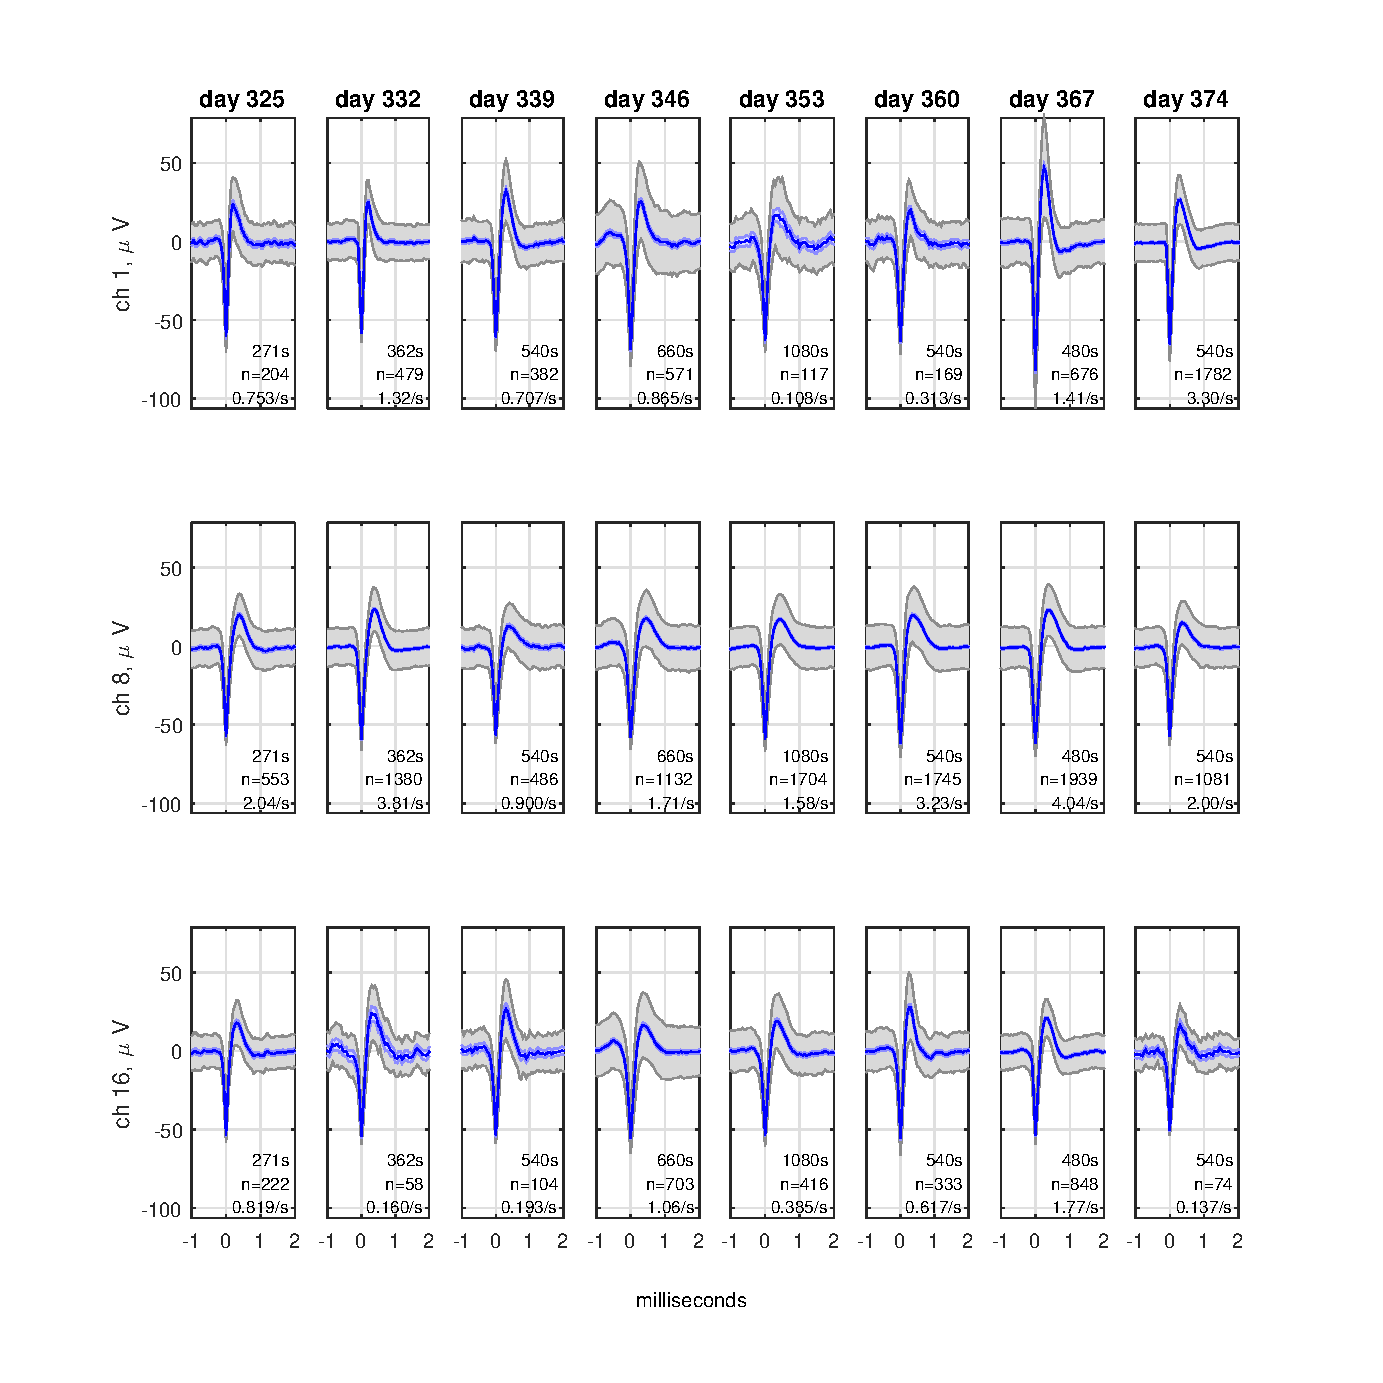
\includegraphics[width=\textwidth]{XSpikeRecording}
  \caption{Some of the electrodes in Area X record spontaneous spikes a year after implantation.  Column titles show the day post-surgery and the number of seconds of recorded data.  Each row is one electrode (shown here: only the three most stable channels out of the 16).  Legends show the number of seconds of the recording, the number of spikes, and mean spike rate.  The grey shaded region is standard deviation, and the blue shaded region is the 95\% confidence interval for the mean.}
  \label{fig:XSpikeRecording}
\end{figure}


\subsection{Stimulation}

\subsubsection{Minimising stimulation voltage}

Some CSCs were better at triggering an antidromic response than others.  From the $2^{11}$ possible CSCs we chose 32 (30 randomly, and the two that treated all electrodes identically).  For each CSC, we performed a threshold scan to find the minimum current needed to trigger a response.  When this current was found, we performed a voltage scan to find the maximum potential on any electrode.  We tested each CSC five times on an anesthetised bird.  Results are shown in \fig{fig:VoltageVsCSC}.  The best CSCs resulted in a maximum voltage of around 1 V, while the worst were over 2.5 V.  Perhaps surprisingly, the CSCs that sent identical pulses to all 11 electrodes were among the worst performers, with our simple search revealing CSCs that kept voltages far lower.

The maximum-likelihood fits to the voltage sweep data (green errorbars in \fig{fig:VoltageVsCSC}) consistently yield slighly higher threshold voltages than those measured using the search.  This is because whereas the maximum-likelihood fit computes the voltage required in order to obtain a response with 50\% probability, the threshold search, which guided data acquisition in realtime, looks for any significant correlation between the responses in each spike train, which is detectable well before the stimulation achieves a 50\% response rate.

\noprint{FIXME: The following caveat doesn't apply to lw95rhp-2015-12-04: Each threshold scan terminated when a stimulation voltage over 3 V was detected, so for some datasets (e.g. lw95rhp-2015-12-09) we were unable to acquire all five measurements for some CSCs, and thus they are worse than the figure shows.}  

\begin{figure}
  % plot_max_voltage_bar.m, reanalyse_thresholds.m
  % lw95rhp-2015-12-04 (data also available on -09 and lw85ry-2015-12-17)
  % width 7 in, height 6 in, fonts auto
  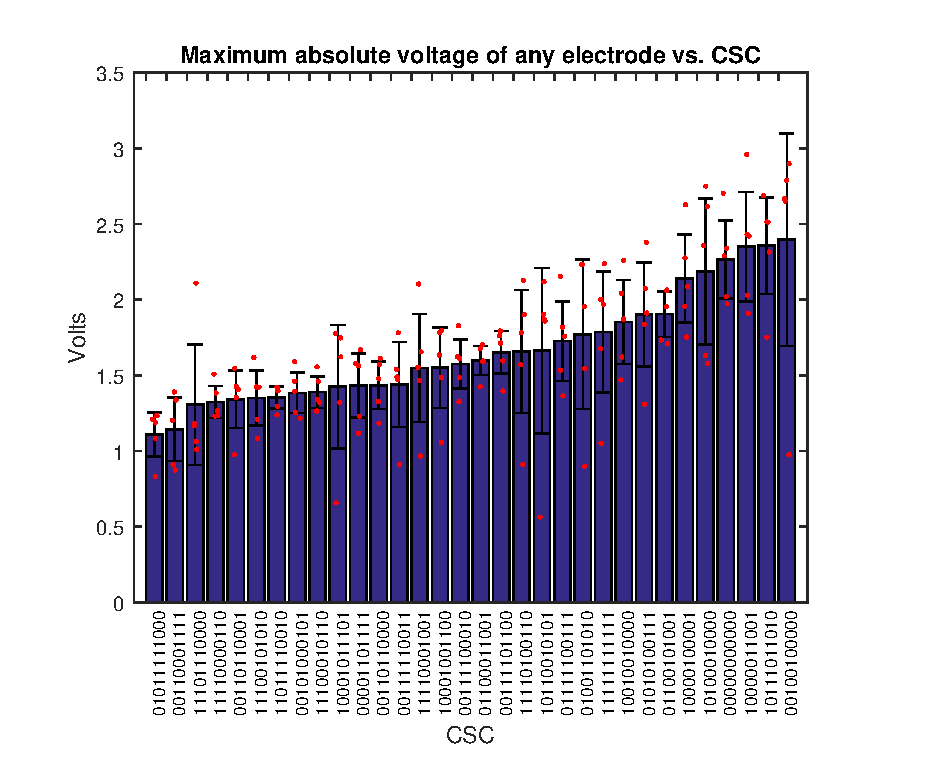
\includegraphics[width=\textwidth]{VoltageVsCSC}
  \caption{The peak Area X stimulation voltage required in order to achieve biologically effective levels of stimulation in HVC varies with different current-steering configurations.  Here are 32 different configurations, over 5 trials each, taken 214 days post-surgery.  The X axis lists the configuration (each of the 11 active electrodes delivers a positive-first ``0'' or negative-first ``1'' current-controlled pulse).  The Y axis shows the maximum voltage across any electrode for the given CSC at the lowest current that evoked a reliable response.  Red dots show the voltage results for each trial, and error bars are 95\% confidence intervals (n=5).  Green bars show maximum-likelihood sigmoid fits for the voltage required to induce 50\% probability of response using a completely separate analysis of the data (see Methods), also as 95\% confidence intervals (when the lines would have spanned the whole range of the graph, they have been omitted for clarity), and with crossbar marker at the mean, with marker size chosen to give an approximate sense of confidence.}
  \label{fig:VoltageVsCSC}
\end{figure}

\subsubsection{Controlling the antidromic response}

\begin{figure}
  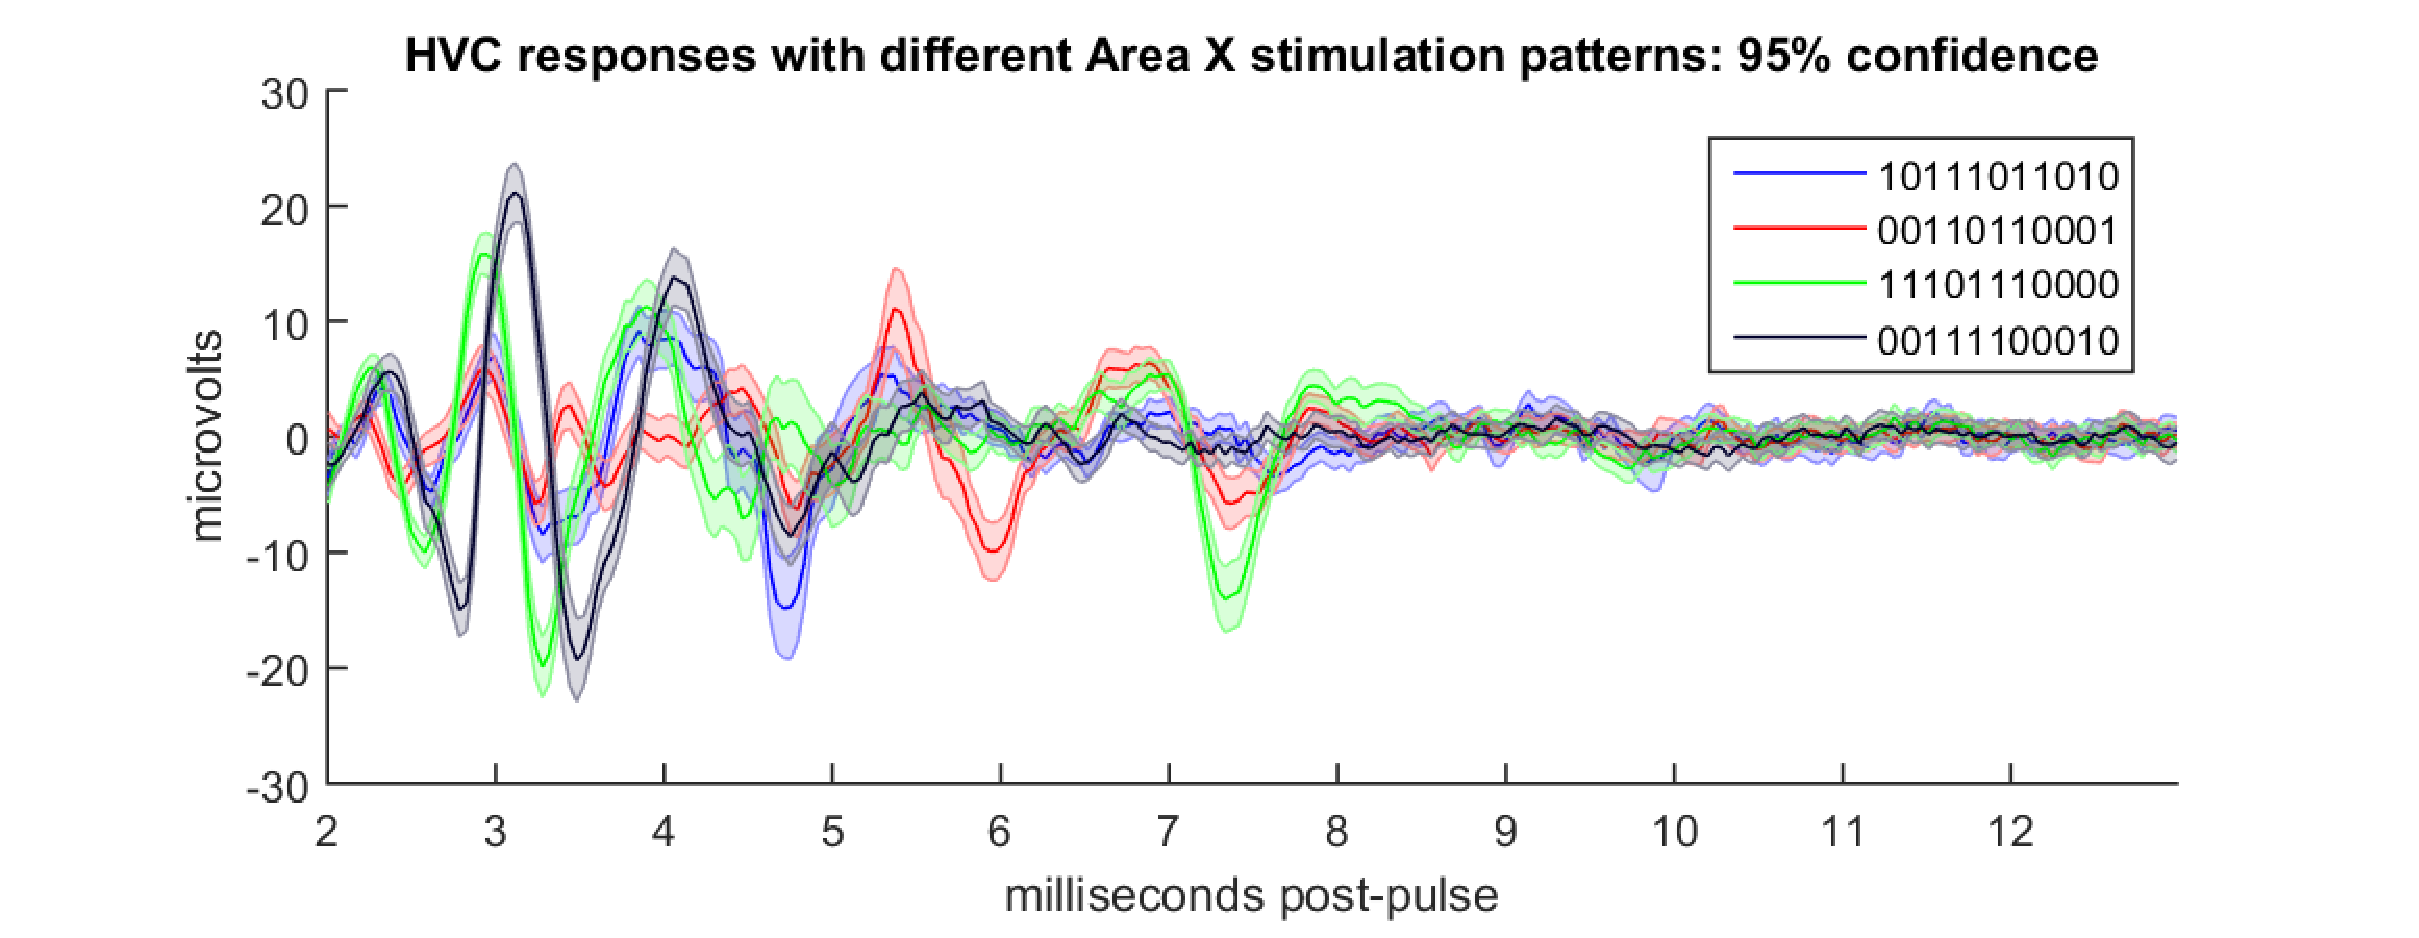
\includegraphics[width=\textwidth]{HVCresponseVsCSC}
  \caption{Different CSCs delivered to Area X can induce different responses antidromically in HVC.  Here are four of the most distinct responses to four of the 32 CSCs shown in \fig{fig:VoltageVsCSC}.  Shading is 95\% confidence, n=198.}
  \label{fig:HVCresponseVsCSC}
\end{figure}


\section{Discussion}

\subsection{Steering}

\cite{Jepson2014steering_in_retina} showed good capacity to control stimulation by steering current between electrodes in monkey retina, allowing targeting of neurons on a smaller scale than the electrode spacing.  The demonstration of fine control is compelling, but whether or not the locally linear predictive response model that they found effective in retina would be extensible to regions with greater lateral connectivity is unknown.

\cite{Histed2009stimulation} showed that injecting current into tissue causes neurons whose axons are very close to the stimulation site to fire, rather than neurons whose bodies are at greater distances.  As a result, the set of neurons that respond to a stimulation pulse is highly sensitive to electrode location, but has spatial extent similar to that of the neuron's dendritic tree.  Furthermore, they showed that neurons stimulated in this manner seldom stimulate downstream neurons synaptically.

Splaying electrode arrays with learning stimulation software may be able to exploit these properties.  First consider each of the $n$ electrodes in our array separately.  $n$ sites stimulated at a given current gives $n$ different random sets of $k_n$ neurons that will fire, and increasing the current changes the size of $k$.  There may exist multiple downstream neurons $y$ such that directly-stimulatable neurons from several of our $n$ sets synapse onto $y$.  This creates a search problem: how to stimulate the $n$ sets in a way that reliably stimulates $y$ enough to cause it to spike?  This requires search over current delivered to each group in $n$ in order to control which neurons are recruited, and timing of stimulation delivery to each group in $n$, so that the downstream neuron is reliably triggered.  Different values of current and timing delivered into the $n$ groups may trigger different downstream neurons, so the search problem is: find as many different downstream neurons as possible.

Furthermore, it seems likely that directly-stimulatable neurons may synapse onto others that are directly-stimulatable, once or $r$ times removed.  This suggests a further dynamic for the timing search, in which different timings for stimulating the $n$ sets may trigger different firing sequences (\cite{Jepson2014steering_in_retina} proposes a related mechanism in the context of current steering in retina).  This enlarges the space of inducible dynamics considerably, and suggests the possibility of inducing Hebbian learning.

Whereas Histed used single electrodes, we use miltichannel arrays.  Rather than a 16-channel array providing $n=16$ groups of neurons, different current-steering configurations may lead to a much higher value of $n$.  For such an electrode there are $2^{16}$ current-steering configurations even without manipulating current pulse magnitude or timing.

\subsection{Ongoing Learning}

The best clinical outcomes require about 20 hours\marginpar{Now where did I read this\dots?} of tuning time, involving multiple patient visits to a clinic.

\subsection{Power}

Another limitation of DBS systems is power use: even with on-demand therapy, the currents required in order to achieve good clinical outcome drain power fast.  Small electrodes that drastically reduce scarring allow stimulation currents several orders of magnitude lower than state-of-the-art systems, and even if current steering does not allow realtime therapy optimisation, it appears to allow further optimisation of power usage.

\bibliography{birds}

\end{document}

